\usetikzlibrary{patterns}
\usepackage{framed}
\usetikzlibrary{decorations.pathmorphing}
\mode<presentation>
{
  \usetheme{CambridgeUS}
  \usecolortheme{whale}
  \usecolortheme{lily}

  \setbeamercovered{transparent}
  \usefonttheme[onlymath]{serif}
}

\title[Root Locus I] % (optional, use only with long paper titles)
{\course: \RootLocusIName\license}

\subtitle
{} % (optional)

\author[\instructorshort]% (optional, use only with lots of authors)
{\instructorlong\credits}
%{T. Vincent\inst{1} \and S.~Another\inst{2}}
% - Use the \inst{?} command only if the authors have different
%   affiliation.

\institute[\instituteshort] % (optional, but mostly needed)
{\institutelong}


\date % (optional)
{Lecture \RootLocusINumber}



% If you have a file called "university-logo-filename.xxx", where xxx
% is a graphic format that can be processed by latex or pdflatex,
% resp., then you can add a logo as follows:

%\pgfdeclareimage[height=1.1cm]{university-logo}{UniversityLogo}
%\logo{\pgfuseimage{university-logo}}



% Delete this, if you do not want the table of contents to pop up at
% the beginning of each subsection:
%\AtBeginSection[]
%{
%  \begin{frame}<beamer>{Outline}
%    \tableofcontents[currentsection,currentsubsection]
%  \end{frame}
%}


% If you wish to uncover everything in a step-wise fashion, uncomment
% the following command:

%\beamerdefaultoverlayspecification{<+->}


\begin{document}

\begin{frame}
  \titlepage
\end{frame}

\mode<article>{
\maketitle
\tableofcontents
}
%\section{\color{red}{Section notes to self - delete before posting}}
%\begin{itemize}
%	\item \color{red}{need to import content, QY, and HW questions from Root Locus II (now an 'X' article)}
%	\item \color{red}{emphasize Matlab-based design after going through the basics}
%\end{itemize}

%\section{Fundamental Equations of Proportional Control} % moved to appendix
\section{Root Locus Motivation}

When designing controllers, it can be useful to get a sense for where the possible closed-loop poles could lie so that we can determine if our controller structure is reasonable given the design specifications (e.g., to achieve the desired transient specifications in Lecture~\HigherOrderResponseNumber:~\HigherOrderResponseName). The \textit{root locus} is a tool that allows us to visualize these closed-loop pole locations without having to recalculate them for a wide variety of controller gains. It is also useful for letting us see easily whether the closed-loop system is in danger of instability. These considerations lead us to our design question.

\begin{frame}{Design Question:}
What closed-loop poles are achievable by varying the gain $K$ in the feedback system below for a given plant $G(s)$, sensor $H(s)$, and basic controller structure $\bar{C}(s)$?
\begin{center}
	\input{figures/pfeedback0.tex}
\end{center}
\end{frame}

Using our block diagram simplification rules for a feedback loop, the closed-loop transfer function is
\[
\frac{Y(s)}{R(s)} = T(s) = \frac{K\bar{C}(s)G(s)}{1+KL(s)}
\]
where $L(s)=\bar{C}(s)H(s)G(s)$ is called the ``loop gain'' (not the closed-loop transfer function) and $\bar{C}(s)$ represents some type of controller (e.g., some variation of PID) from which a gain $K$ has been factored out so we can evaluate its effect. The poles of this closed-loop transfer function will be the values of $s$ for which
\begin{equation} \label{eq:syscl}
T(s) = \frac{K\bar{C}(s)G(s)}{1+KL(s)} = \infty
\end{equation}
and a plot of these possible poles as $K$ goes from $0$ to $\infty$ is called a root locus plot. We achieve $T(s) = \infty$ in (\ref{eq:syscl}) by setting the denominator equal to zero, i.e., 
\begin{align*}
1+KL(s)&=0 \\
\Rightarrow KL(s)&=-1.
\end{align*}

Let's take an example with a simple plant system to illustrate the root locus, first without technology. 

\begin{example} \label{ex:motivating}
	
	Determine the possible closed-loop poles for the following proportional control system as $K$ goes from $0$ to $\infty$ .
	\begin{center}
		\input{figures/pfeedbackexample2ndorder.tex}
	\end{center}
	First, note that by comparing this example to the more general one above, we have a system with plant $G(s)=\frac{1}{s^2}$, $\bar{C}(s)=1$ (as expected for proportional control, the controller has no poles or zeros), and $H(s)=1$. Using our block diagram simplification rules, the closed-loop transfer function is
	\[
	T(s)=\frac{Y(s)}{R(s)} = \frac{K\frac{1}{s^{2}}}{1+K\frac{1}{s^{2}}} = \frac{K}{s^{2}+K}
	\]
	The closed-loop poles are determined by the roots of the denominator
	\[
	s^{2}+K=0
	\]
	In this case, it is clear that the closed-loop poles are given by
	\[
	s = \pm j\sqrt{K}
	\]
	By varying $K$, we can select different poles; for example, when $K=9$, the closed-loop poles are $s_{1,2}=\pm j3$. No matter what the value of $K>0$, the closed-loop poles will always be purely imaginary. That is, the closed-loop poles will always lie along the imaginary axis for this plant $G(s)=\frac{1}{s^2}$ with proportional control.
\end{example}

In this lecture, we'll be looking at what we need to know in order to use root locus for control design. %In particular, we'll be looking at 
%\begin{itemize}
%	\setlength{\itemsep}{0pt}
%	\setlength{\parskip}{0pt}
%	\setlength{\parsep}{0pt}
%	\item The total number of loci (plural of locus),
%	\item The locations of the loci on the real axis,
%	\item The starting and ending points of each locus, and
%	\item The angles at which the loci approach infinity magnitude, which helps us to know whether it is possible for the closed-loop poles to enter the right-half plane, making $T(s)$ unstable.
%\end{itemize}


\section{Root Locus Plotting and Features}
Using a computer, we can easily visualize all of the closed-loop poles achievable by finding all the solutions of the equation $KL(s)=-1$ for various values of $K$. This plot is called a {\em root locus}, since the closed-loop poles are the roots of the equation $KL(s)+1=0$. 

\begin{example} \label{ex:matlab1}
Let's return to Example~\ref{ex:motivating}~and look at the root locus plot in Matlab. We can use the \textsc{Matlab} command \texttt{rlocus} to plot the root locus. This command specifically expects the system to be a negative feedback configuration with a proportional gain $K$ (such as the block diagram given above). The only thing we need to tell it is the loop gain %system under control, also called the {\em open loop transfer function}. In this case, it is 
\begin{align*}
L(s) &= \bar{C}(s)G(s)H(s) \\
&=\frac{1}{s^{2}}
\end{align*}

\begin{frame}{Plotting the root locus using \textsc{Matlab}}
\texttt{\\<all>
\noindent>> s = tf(\T\rule{0pt}{0pt}s\T); \% note: another way to define a TF using s as a variable \\<all>
>> L = 1/s\^{}2\\<all>
>> rlocus(L)\\<all>}
\begin{center}
\mode<article>{\includegraphics[width=4in]{figures/rlocusexample0}}
\mode<presentation>{\includegraphics[width=3in]{figures/rlocusexample0}}
\end{center}
\end{frame}

Each colored line represents the location that the closed-loop poles {\em could be} for a proper choice of $K>0$. Note that both lines are on the imaginary axis, and agree with our calculation of closed-loop poles $s=\pm j\sqrt{K}$. The `x' at the origin is actually two `x' markers, one on top of the other, which represent the poles of $L(s)$, i.e., the poles of $\bar{C}(s)$, $G(s)$, and $H(s)$. As expected from our analysis in Example~\ref{ex:motivating}, these loci encompass the imaginary axis. 



\end{example}


\begin{example} \label{ex:control}
	Consider again the system shown in Example~\ref{ex:motivating}. Given this plant and the specified proportional controller, is it possible to satisfy a settling time requirement $t_s < 4.6$~s in response to a step input?
	
	Based on this settling time constraint, we need the closed-loop damping and natural frequency $\zeta \omega_n > 1$, which is equivalent to saying we need the closed-loop poles to be to the left of a vertical line with real part equal to -1 in the complex plane. 
	
	\begin{frame}{Settling Time Requirement for Example}
	\begin{center}
		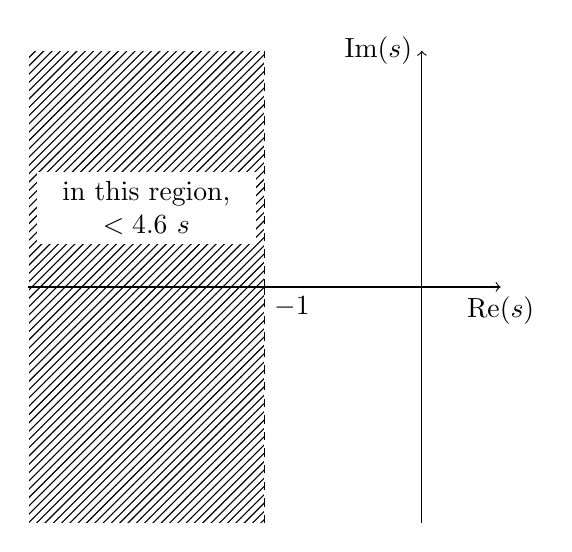
\begin{tikzpicture}

\draw[pattern=north east lines,draw=white] (-5,-3) rectangle (-2,3);
\draw[dashed] (-2,-3) -- (-2,3);
\draw[->] (-5,0) -- (1,0) node[below] {$\mbox{Re}(s)$};
\draw[->] (0,-3) -- (0,3) node[left] {$\mbox{Im}(s)$};
\draw (-2,-.1) -- (-2,.1);
\draw (-2,0) node[below right] {$-1$} (135:2);
\draw (-3.5,1) node[fill=white] {\begin{minipage}{1in}\begin{center}in this region, $\ts < 4.6~s $\end{center}\end{minipage}};
\end{tikzpicture}
	\end{center}

By comparing the root locus (closed-loop poles on the imaginary axis) from Example~\ref{ex:matlab1} to the allowable region for the closed-loop poles (real part < -1) here, it's clear that the possible closed-loop poles do not enter the desired region for this settling time specification. Therefore, we would not be able to satisfy the settling time specification using proportional control and would need to use a different kind of controller $\bar{C}(s)$, motivating Lecture~\RootLocusIINumber.
\end{frame}

\end{example}

Let's look at a final motivating example with a more complicated plant system $G(s)$ to see some other characteristics of root locus plots.

\begin{example} \label{examp:rlocus} Plot the root locus for the following proportional control system
\begin{center}
\input{figures/pfeedbackexample2.tex}
\end{center}

The \textsc{Matlab} command \texttt{rlocus} will plot the root locus:

\begin{frame}{Plotting the root locus using \textsc{Matlab}}
\texttt{\\<all>
\noindent>> s = tf(\T\rule{0pt}{0pt}s\T);\\<all>
>> G = (s+6)/((s+1)*(s+10)*(s\^{}2+10*s+50))\\<all>
>> rlocus(G)\\<all>}
\begin{center}
\mode<article>{\includegraphics[width=4in]{figures/rlocusexample}}
\mode<presentation>{\includegraphics[width=3in]{figures/rlocusexample}}
\end{center}
\end{frame}

Again, note that the {\em open} loop gain transfer function $L(s)$ is given to the root locus command. 
\end{example}

Each colored line represents the set of locations that the closed-loop poles {\em could be} for different choices of $K>0$. By clicking on one of the root loci lines, \textsc{Matlab} will tell us what gain $K$ would place the closed-loop poles at that location (in this example, $K=241$), as well as the closed-loop pole location and associated damping $\zeta$, predicted percent overshoot, and natural frequency $\omega_n$ are associated with that pole location. 

\newpage
\begin{frame}{Pole Location Information}
\begin{center}
\includegraphics[width=4.5in]{figures/rlocusexample2}
\end{center}
\end{frame}

Notice in this example that we have four total loci, two of which are on the real axis and two of which go off towards magnitude $\infty$ at some angles, crossing into the right half plane, which indicates the possibility for the closed-loop system to be unstable for certain values of $K$. 

Together, these examples can motivate the need to learn some rules for root locus features that can help with design of $\bar{C}(s)$, even if we still use computers to do most of the plotting. Knowing the rules will also help us to check our computer-based results to make sure we've implemented everything correctly. 

%\section{Root Locus Features}

%Although computers are available to plot the complete root locus, there are some simple rules that allow us to sketch the main features, which helps us to double-check our computer results. Knowing these rules will also give us insight to know what we might want to do with our controller $\bar{C}(s)$ in order to improve our closed-loop pole options.  

Many rules are available for sketching root locus, but in \course, we will limit ourselves to four questions:

\begin{frame}{Four Questions for Root Locus Features}
\begin{itemize}
\setlength{\itemsep}{0pt}
\setlength{\parskip}{0pt}
\setlength{\parsep}{0pt}
\item How many loci will we have? 
\item Where do the loci begin ($K=0$) and end ($K=\infty$)? 
\item When do we have loci on the real axis? 
\item At what angles do the loci approach magnitude $\infty$? (Especially relevant to whether they enter the right half plane, meaning the closed-loop system becomes unstable.)
\end{itemize}
\end{frame}

\subsection{Root Loci - How Many?}

First, let's determine how many root loci there are - in other words, how many poles will the closed-loop system have? Our fundamental equation (refer to (\ref{eq:syscl})) states that the closed-loop poles satisfy
\begin{equation} \label{eq:KL(s)}
KL(s) +1 = 0
\end{equation}
Let's suppose the loop gain is rational and can be expressed as a ratio of polynomials $N(s)$ and $D(s)$. 
\[
L(s) = \frac{N(s)}{D(s)}
\]
In other words, $N(s)$ is the numerator polynomial, whose roots define the open loop zeros, while $D(s)$ is the denominator polynomial, whose roots define the open loop poles. We will assume that like all physical systems $G(s)$ is {\em proper}, so that the number of zeros (the order of the numerator, $N(s)$) is less than or equal to the number of poles (the order of the denominator $D(s)$). 

Now, the closed-loop poles satisfy
\[
K\frac{N(s)}{D(s)} + 1 =0
\]
or, multiplying both sides of the equation by $D(s)$,
\begin{equation}\label{eq:KN+D}
KN(s)+D(s) = 0
\end{equation}
This is a polynomial whose roots define the closed-loop poles. The number of roots equals the order of a polynomial, and the order of this polynomial will be the same as the highest order of $N(s)$ and $D(s)$, which will be $D(s)$ as long as the open loop system is proper (as we assume in this class). Thus:
\begin{center}
\fbox{\begin{minipage}{5in}The number of closed-loop poles is the same as the number of open loop poles - The number of root loci is equal to the number of open loop poles.\end{minipage}}
\end{center}

\subsection{Beginnings and Endings}
Where are the poles along the loci when $K$ is small, i.e., when they \textit{begin}? Where do they go when $K$ is big, i.e., when they \textit{end}? We can determine where the loci begin and end by continuing our analysis of Equation~(\ref{eq:KN+D}), the roots of which are the closed-loop poles.
%with the modified closed-loop pole equation
%\[
%KN(s)+D(s)=0
%\]
%we derived above. 
Suppose $K$ is really small. Then (\ref{eq:KN+D}) can be approximated as
\[
KN(s)+D(s) \approx D(s).
\]
In other words, when $K$ is very small -- where the loci begin -- the closed-loop poles are given by a polynomial which is approximately equal to the open loop denominator. Thus,
\begin{center}
\fbox{The closed-loop root loci {\em start} at the open loop poles}
\end{center}

Now suppose $K$ is really big, i.e., approaching the ends of the loci. Then
\[
KN(s)+D(s) \approx KN(s).
\]
Now the closed-loop poles are given by a polynomial that is approximately equal to the open loop numerator. Thus, 
\begin{center}
\fbox{\begin{minipage}{5in}The closed-loop root loci {\em end} at the open loop zeros. If the number of zeros is less than the number of poles, some closed-loop poles go to infinity.\end{minipage}}
\end{center}

\begin{example} 
	Let's look again at the root locus for the feedback system of Example \ref{examp:rlocus}. The open loop transfer function was:
\[
L(s) = \frac{s+6}{(s+1)(s+10)(s^{2}+10s+50)}
\]
which has
\begin{itemize}
\item zeros: -6
\item poles: -1, -10, $-5+5j$, $-5-5j$.
\end{itemize}
Since there are 4 open loop poles, there will be 4 closed-loop poles, and we expect 4 root loci. One of those root loci will end (i.e. with large $K$) at $s=-6$, while the other three will go off to infinity. The plots below show this root locus plot with closed-loop pole values indicated by triangles for three different values of $K$. Note that when $K=5000$, the closed-loop poles are in the right half plane, indicating that the closed-loop system is unstable. 

\begin{frame}{Root Locus with closed-loop pole overlay}
\includegraphics[width=2in]{figures/rlocusexample3}
\includegraphics[width=2in]{figures/rlocusexample4}
\includegraphics[width=2in]{figures/rlocusexample5}
\end{frame}
\end{example}

\subsection{Location of Loci on Real Axis}
Many root locus plots show that one or more locus lies on the real axis. Because of the properties of the angle of a complex number and the fact that complex poles (and zeros) always appear in complex conjugate pairs, we can dismiss the complex poles and zeros from our analysis to determine where the loci lie on the real axis (see Appendix B for details).

Let's indicate a pole of the loop gain $L(s)$ by $p_i$; in other words, $L(p_i)=\infty$ since $p_i$ is a root of the denominator of $L(s)$. Suppose a pole $p_{i}$ is real but to the left of a possible closed-loop pole location $s$ (i.e., a possible root of $T(s)$ from (\ref{eq:syscl})).
\begin{center}
\begin{tikzpicture}
\draw[->] (-5,0) -- (1,0) node[below] {$\mbox{Re}\{s\}$};
\draw[->] (0,-2) -- (0,2) node[left] {$\mbox{Im}\{s\}$};
\draw (-2,0) node[circle,draw,fill=blue,inner sep=0pt,outer sep=0pt] (s) {\rule{3pt}{0pt}} node[above left] {$s$}; 
\draw (-4,0) node[inner sep=0pt,outer sep=0pt] (z1) {\textsf{x}} node[below right] {$p_{i}$};
\draw[->,thick] (z1) -- (s);
%\draw (z1) ++(.4,0) arc (0:225:.4);
\draw (z1) ++(.5,.5) node {$0^{\circ}$};
\end{tikzpicture}

\end{center}
Since the angle from the pole $p_i$ to this location $s$ is zero, poles and zeros to the left of $s$ are {\em not} significant when calculating $\angle L(\bar{s})$.

Finally, suppose $p_{i}$ is real, but to the right of $s$
\begin{center}
\input{figures/realright.tex}
\end{center}
For each pole or zero to the right of $s$, the angle from the pole $\times$ to this location $s$  is $180^{\circ}$. Referring back to Equation~(\ref{eq:KL(s)}), since $\angle K = 0^\circ$ (since $K>0$), we know that loci must satisfy $\angle L(\bar{s})=\pm 180^{\circ}$

Conclusion:
\begin{center}
\fbox{\begin{minipage}{5in} When $\bar{s}$ is real, $\angle L(\bar{s}) = -180^{\circ}$ (and thus $\bar{s}$ is on the root locus) whenever there is an {\em odd} number of real poles and zeros of $L(s)$ to the right of $\bar{s}$. \end{minipage}}
\end{center}
An alternative but commonly-used way of stating the same conclusion is
\begin{center}
	\fbox{\begin{minipage}{5in} Loci exist on the real axis to the left of an {\em odd} number of real poles and zeros of $L(s)$. \end{minipage}}
\end{center}


For example, consider the root locus we plotted in Example~\ref{examp:rlocus}
\begin{frame}{Root locus on the real axis}
\begin{center}
\includegraphics[width=4in]{figures/rlocusexample}
\end{center}
\end{frame}
We can interpret this plot as follows. 
\begin{enumerate}
\setlength{\itemsep}{0pt}
\setlength{\parskip}{0pt}
\setlength{\parsep}{0pt}
	\item Moving an imaginary cursor point from the far right side of the plot back towards the left on the real axis, there is no root locus when $s>-1$ since we have not yet passed any poles or zeros, meaning that these points on the real axis are to the left of 0 -- an even number -- real poles and zeros. 
	\item Continuing to move leftwards, between $-6<s<-1$ the root locus exists in this region because it is to the left of the real pole at -1. 
	\item Continuing to move leftwards, for the region $-10<s<-6$, we are now to the left of one (real) pole and one (real) zero for a total of two, which is even, so no root locus.
	\item  Finally, for $s<-10$, we are now to the left of three (real) poles and zeros, so the root locus occurs again.\footnote{Another way of stating the information in this list: 
		There is no root locus for $s>-1$, as there are no poles and zeros to the right. For $-6<s<-1$, there is one (real) pole to the right and the root locus exists in this region. For $-10<s<-6$, there is one (real) pole and one (real) zero to the right for a total of two, which is even, so no root locus. Finally, for $s<-10$, three (real) poles and zeros are to the right, so the root locus occurs again.} % KEJ Note: students found the original explanation confusing so I re-wrote it for my section.
\end{enumerate}

\subsection{Asymptotic Loci}
When the number of finite zeros of $L(s)$ is less than the number of poles of $L(s)$ -- in other words, when $L(s)$ is strictly proper -- we have seen that one or more of the root loci go off to infinity. As they do this, they will approach asymptotes that are easy to calculate. As before, we assume $n$ poles and $m$ zeros. 
\begin{itemize}
\item Center of asymptote
\[
\sigma_{A} = \frac{\sum \mbox{poles of $L(s)$} - \sum \mbox{zeros of $L(s)$}}{n-m}
\]
\item Angles of asymptotes
\[
\phi_{A} = \frac{2q+1}{n-m}180^{\circ} \quad q = 0,1,\cdots,n-m-1
\]
\end{itemize}
\begin{example} Find the asymptotes for Example \ref{examp:rlocus}. With 
\[
L(s) = \frac{s+6}{(s+1)(s+10)(s^{2}+10s+50)}
\]
we can calculate
\[
\sigma_{A} = \frac{(-1-10-5-5) - (-6)}{4-1} = \frac{-15}{3} = -5
\]
and
\[
\phi_{A} = \frac{2q+1}{3}180^{\circ} = 60^{\circ},180^{\circ},300^{\circ}
\]
\end{example}
\begin{frame}{Root Locus Asymptotes}
\begin{center}
\includegraphics[width=4.5in]{figures/rlocusasymptotes}
\end{center}
\end{frame}

A key fact from this study is that two of the asymptotes, specifically the ones with angles of $60^\circ$ and $300^\circ$, will enter the right half plane (RHP) no matter where they start. This means that we will need to be careful about our choice of $K$, since at some point $K$ will be large enough to cause the closed-loop system to be unstable. 

%\section{Application Example}
%%\textit{Related to general concepts in the lecture}
%
%\noindent Consider again the wind turbine system in feedback with (preliminary) controller \(C(s) = K\) (a constant) shown in Figure \ref{fig:controlLoop}, where
%\begin{equation*}
%	G_2(s) = \frac{-21.201(s^2+0.04283s+6.509)}{(s+0.2867)(s^2+0.2996s+6.477)}
%\end{equation*}
%
%\begin{figure}
%	\begin{center}
%		\includegraphics[width = 4in]{figures/ControlLoop.png}\\
%		\caption{Wind turbine plant with feedback control loop and disturbance input.}
%		\label{fig:controlLoop}
%	\end{center}
%\end{figure}
%
%\noindent Note that we have an unusual case here: the plant \(G_2(s)\) is negative, which means that as the wind turbine's blade pitch angle \(\beta\) increases the rotor speed \(\omega\) decreases. Therefore, we use a negative gain \(K\) in our controller, which maintains stability and allows us consistency with the other class examples. 
%
%The root locus for this case is shown in Figure \ref{fig:rootLocusP}. Since all of the loci are in the left half plane, we expect to be able to increase the proportional gain as high as we want without causing closed-loop instability. In other words, as long as our reference speed \(\omega_{ref}\) is bounded, we can be assured that our rotor speed will be bounded (not go to infinity). An unbounded rotor speed would eventually destroy the wind turbine.\\
%
%\begin{figure}
%	\begin{center}
%	\includegraphics[width = 4in]{figures/RootLocus.png}\\
%	\caption{Figure 2: Root locus for proportional controller case.}
%	\label{fig:rootLocusP}
%	\end{center}
%\end{figure}
%
%
%
%\noindent \textbf{Question:} How would this answer change if instead of a proportional controller we used a PI controller such as
%\begin{equation*}
%	C(s) = K_p + \frac{K_I}{s} = K_p \frac{S+\frac{K_I}{K_p}}{s}
%\end{equation*}
%\noindent (with \(K_p\) < 0 for the same reason described above)? 
%
%\noindent \textbf{Answer:} The PI controller adds a zero at \(-K_I / K_p\) and a pole at zero. For one example, the root locus would appear as shown in Figure \ref{fig:rootLocusPI}, which still guarantees stability for any (negative) value of \(K_p\).\\
%
%\begin{figure}
%	\begin{center}
%	\includegraphics[width = 4in]{figures/RootLocus2.png}\\
%	\caption{Sample root locus for PI controller, with controller zero set to -1.}
%	\label{fig:rootLocusPI}
%	\end{center}
%\end{figure}
%
%
%\noindent \textbf{Question:} What could we do with the PI controller to force an unstable closed-loop system?


\section{Lecture Highlights}
The primary takeaways from this article include
\begin{enumerate}
\setlength{\itemsep}{5pt}
\setlength{\parskip}{0pt}
\setlength{\parsep}{0pt}
\item The loci (plural of ``locus'') in a root locus plot are the set of all possible closed-loop poles as a gain $K$ varies from zero to infinity. 
\item The root locus plot is drawn starting with the open loop poles and zeros and then applying some sketching rules or using the \texttt{rlocus} command in Matlab.
\item For this course, you should be able to determine the number of loci, where they begin ($K=0$) and end ($K=\infty$), where they lie on the real axis, and the centers and angles of the asymptotes that the loci approach.
\end{enumerate}

\section{Quiz Yourself}

\subsection{Questions}

\begin{enumerate}
\setlength{\itemsep}{5pt}
\setlength{\parskip}{0pt}
\setlength{\parsep}{0pt}
\item Sketch the root locus with respect to $K$ for the closed-loop system with transfer function denominator $1+KL(s)=0$ for
\[
L(s)=\frac{s+2}{s(s+1)(s+5)(s+10)}.
\]
Be sure to find where the root locus exists on the real axis, and the asymptotes. After completing each hand sketch, verify your results using the \textsc{Matlab} commands
\texttt{\\
>> sys=tf(num,den);\\
>> rlocus(sys);\\
}
Note that \texttt{num} and \texttt{den} should contain the numerator and denominator coefficients, respectively, of the open loop system.
\item Determine  how the closed-loop poles of the following feedback system change as $K$ varies.
\begin{frame}{Root Locus Example Problem 1}
\begin{center}
	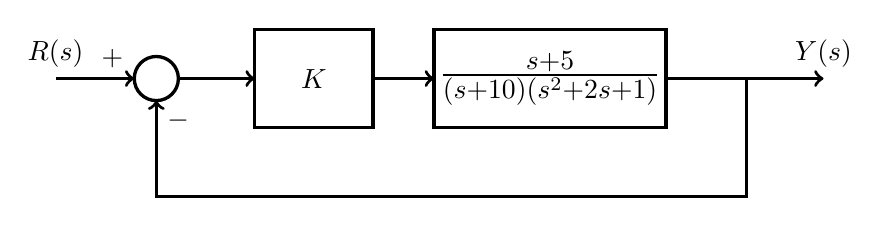
\begin{tikzpicture}[inner sep=0pt,outer sep=0pt,very thick,
sysblock/.style={draw,rectangle,inner sep=2pt,minimum width=1.5cm,minimum height=1.25cm,very thick}]

\draw (0,0) node[draw,circle] (sum) {$\rule{0pt}{16pt}$};
\draw (2.0,0) node[sysblock] (a) {$K$};
\draw (5,0) node[sysblock] (b) {\Large $\frac{s+5}{(s+10)(s^{2}+2s+1)}$};
\draw (b.0) ++(1,0) node (c) {};

\draw[<-] (sum.180) node[above left=4pt] {$+$} -- ++(-1,0) node[above=4pt] {$R(s)$};
\draw[->] (sum.0) --  (a.180);
\draw[->] (a.0) -- (b.180);
\draw[->] (b.0) -- ++(2,0) node[above=4pt] {$Y(s)$};
\draw[->] (c.0) -- ++(0,-1.5) -| (sum.-90) node[below right=4pt] {$-$};

\end{tikzpicture}
\end{center}
\end{frame}

\end{enumerate}
%\pagebreak
\vspace{1in}

\subsection{Solutions}
\begin{enumerate}
\setlength{\itemsep}{5pt}
\setlength{\parskip}{0pt}
\setlength{\parsep}{0pt}
\item Notational note: loci on the real axis are indicated by squiggly lines so they can be seen over the axis line itself. \rule{0pt}{12pt}\\
\begin{center}
\includegraphics[width=5in]{quizfigures/1asoln}\\
\includegraphics[width=4in]{quizfigures/1bsoln}
\end{center}

\item \begin{itemize}
	\item Step 1: Find and plot poles and zeros
	\begin{itemize}
		\item Poles: -10, -1, -1
		\item Zeros: -5
	\end{itemize}
	
	\item Step 2: Find region on real axis with root locus
	\begin{itemize}
		\item An odd number of poles and zeros to the right for $-10<s<-5$.
	\end{itemize}
	
	\item Step 3: Find Asymptotes and Sketch
	\begin{itemize}
		\item $n$ = number of poles
		\item $m$ = number of zeros
		\item Asymptote center
		\begin{align*}
		\sigma_{A} &= \frac{\sum \mbox{poles} - \sum \mbox{zeros}}{n-m}\\
		& = \frac{-10 -1 -1 -(-5)}{3-1}\\
		& = \frac{-7}{2}
		\end{align*}
		\item Asymptote angles
		\begin{align*}
		\phi_{A} &= \frac{2q+1}{n-m}180^{\circ} \quad q=0, 1, \cdots ,n-m-1\\
		&= \frac{2(0)+1}{3-1}180^{\circ},\;\frac{2(1)+1}{3-1}180^{\circ}\\
		&=90^{\circ},\; 270^{\circ}
		\end{align*}
	\end{itemize}
\end{itemize}

%\begin{frame}{Example 1 Sketch}
\begin{center}
	\includegraphics[width=4in]{figures/pfeedbacksketch3}
\end{center}
%\end{frame}

We can check the sketch against the result in \textsc{Matlab}:\\

%\begin{frame}{Matlab Result}
\texttt{\\<all>
\noindent>> s = tf([1 0],[1]) \% define s as the Laplace variable\\<all>
>> sys = (s+5)/((s+10)*(s\^{}2+2*s+1));\\<all>
>> rlocus(sys)}
\begin{center}
\includegraphics[width=3in]{figures/pfeedbackmatlab3}
\end{center}
%\end{frame}
Notice that the general ideas are the same, but we didn't capture quite the angles of the loci leaving the two real poles at -1 and approaching the asymptotes (which is fine -- that's why we have \textsc{Matlab}).

\end{enumerate}

\section{Appendix A
\label{sec:appendixA}}

This appendix derives some of the ideas behind the root locus tool by asking the question:

\begin{frame}{}
\begin{itemize}
	\item What closed-loop poles are achievable using proportional control?
\end{itemize}
\begin{center}
	\input{figures/pfeedback.tex}
\end{center}
\end{frame}

We can answer this question by finding the closed-loop transfer function, and finding the poles of that transfer function. Using our formula for a feedback loop in a block diagram, the closed-loop transfer function is
\[
\frac{Y(s)}{R(s)} = T(s) = \frac{KG(s)}{1+KL(s)}
\]
where $L(s)=H(s)G(s)$, the loop gain. The poles of this transfer function will be the values of $s$ for which
\[
T(s) = \frac{KG(s)}{1+KL(s)} = \infty
\]
So when will this ratio be infinite? Will this be when the numerator $G(s)$ is infinite (i.e. the open loop poles)? No! Since $G(s)$ appears in both the numerator and denominator, by L'Hopitals rule, the value of $T(s)$ will be $1$, and thus finite. Instead, the closed-loop poles only occur when $1+KL(s)=0$. Or, moving the 1 to the other side, we have the following fundamental relationship for closed-loop poles. 
\begin{fact}
Given a system described by the (open) loop gain transfer function $L(s)$, when using proportional feedback, $s=\bar{s}$ is a closed-loop pole if and only if
\[
\boxed{KL(\bar{s}) = -1}
\]
\end{fact}

Using this relationship, we can test if proportional control can achieve a particular closed-loop pole location

\begin{example}\label{examp1} Can the following control system set one of the closed-loop poles at $\bar{s}=-1+j$?
\begin{center}
	\input{figures/pfeedbackexample1.tex}
\end{center}
To check, we use the test given above:
\begin{align*}
KL(\bar{s}) &= KL(-1+j) \\
&= K\frac{(-1+j)+1}{(-1+j)^{2} +3(-1+j) +1} \\
& = K\frac{j}{1 - 2j -1 -3 +3j +1}\\
& = K\frac{j}{j-2}
\end{align*}
So, does there exist a value of $K$ such that
\[
K\frac{j}{j-2} = -1?
\]
Solving for $K$, we get
\[
K = -\frac{j-2}{j} = -1-2j.
\]
However, we have a problem: the gain that we implement needs to be a real number! Since this is not the case, we can say that proportional control cannot achieve a closed-loop pole at $s=-1+j$.  \qed
\end{example}

\begin{example} Consider the same proportional control system as for Example \ref{examp1}. Can this control system achieve a closed-loop pole at $\bar{s}=-4$?\\

Again, we check by plugging in to $KL(s)$:
\begin{align*}
KL(\bar{s})& = KL(-4) \\ 
& = K\frac{-4+1}{(-4)^{2} + 3(-4) +1} \\
& = K\frac{-3}{16-12+1} \\
& = K\frac{-3}{5}
\end{align*}
So does there exist a $K$ such that $KL(\bar{s})=-1$? In this case, yes, choose $K=\frac{5}{3}$. The difference in this case is that $L(\bar{s})$ is {\em real} \qed
\end{example}

Looking at what we did in the previous examples, we can see that the only way that there exists a real $K$ to achieve closed-loop poles at $\bar{s}$ is if $L(\bar{s})$ is a real number. Usually, we also restrict $K$ to be a positive number so that we maintain a negative feedback loop. This results in the following test:
\begin{fact}
Using proportional control, there exists a $K>0$ to achieve the closed-loop pole $s=\bar{s}$ if and only if $L(\bar{s})$ is real and negative. In other words,
\[
\boxed{\angle L(\bar{s}) = -180^{\circ}}
\] 
\end{fact}
An important aspect of this test is that it is independent of $K$. We don't need to know the gain in order to test if a particular pole location is feasible.

\section{Appendix B}
Why don't complex poles or zeros matter when determining where the root loci lie on the real axis? The complex conjugate symmetry of the poles and zeros makes this easy to answer. We start with our fundamental equation: $\bar{s}$ is on the root locus if
\[
\angle L(\bar{s}) = -180^{\circ}.
\]
If our open loop transfer function $G(s)$ has poles $p_{i}$ and zeros $z_{i}$, then we can write it as
\[
\angle L(s) = \angle \frac{(s-z_{1})(s-z_{2})\cdots(s-z_{m})}{(s-p_{1})(s-p_{2})\cdots(s-p_{n})}
\]
Using the angle property of complex multiplication and division (i.e. $\angle s_{1}s_{2} = \angle s_{1} +\angle s_{2}$, and $\angle\frac{s_{1}}{s_{2}} = \angle s_{1} - \angle s_{2}$,) we can write
\[
\angle L(s) = \sum_{i=1}^{m} \angle (s-z_{i}) - \sum_{i=1}^{n} \angle (s - p_{i}).
\]
What makes this analysis easy is that each of the angles $\angle (s-z_{i})$ and $\angle (s-p_{i})$ can be easily visualized on a pole/zero plot. Given any point $s$ and any other point $z$, the angle $\angle (s-z)$ is given by the angle of the line between the two points, measured at $z$ from a line parallel to the real axis, and shown below.
\begin{center}
	\begin{tikzpicture}
\draw[->] (-1,0) -- (5,0) node[below] {$\mbox{Re}\{s\}$};
\draw[->] (0,-1) -- (0,3) node[left] {$\mbox{Im}\{s\}$};
\draw (3,1) node[circle,draw,fill=blue,inner sep=0pt,outer sep=0pt] (s) {\rule{3pt}{0pt}} node[below right] {$z$}; 
\draw (1,2) node[circle,draw,fill=blue,inner sep=0pt,outer sep=0pt] (z) {\rule{3pt}{0pt}} node[above left] {$s$};
\draw (3.6,1.6) node {$\angle (s-z)$};
\draw (3.4,1) arc (0:150:.4);
\draw[->] (s) -- (z);
\draw[-,dotted] (s) -- ++(1,0); 
\end{tikzpicture}

\end{center}

Let's see what happens when we choose $s$ on the real axis. First, suppose $z$ or $p$ is complex. For concreteness we will use poles, but the same conclusions hold for zeros. Since all complex roots happen in complex conjugate pairs, we can look at these terms in pairs:
\[
\angle(s-p_{i}) + \angle(s-p_{i}^{*}).
\]
Consider the plot below.
\begin{center}
	\input{figures/complexangle.tex}
\end{center}
Looking at the geometry, the angle from one pole is 360  minus the angle from the other pole. Thus, when $s$ is real,
\[
\angle(s-p_{i}) + \angle(s-p_{i}^{*}) = \theta + 360^{\circ} - \theta = 360^{\circ} = 0^{\circ}
\]
Conclusion: complex poles or zeros are {\em not} significant when calculating $\angle G(\bar{s})$.



\end{document}